\documentclass[letterpaper,12pt,fleqn]{article}
\usepackage{matharticle}
\usepackage{mathtools}
\usepackage{amsfonts}
\usepackage{tikz}
\pagestyle{empty}
\begin{document}
Cavallaro, Jeffery \\
Math 279b \\
Homework \#5

\bigskip

\begin{enumerate}
\item $G(n,\frac{1}{2})$ \\
X = number of vertices with degree $<\frac{n}{2}$ \\
Compute $E(X)$

\bigskip

Let $a=\left\{
    \substack{\frac{n-2}{2},\ n\ \mbox{even} \\
              \frac{n-1}{2},\ n\ \mbox{odd}
}\right.$

Let $X_v=deg(v)\le a$

\begin{eqnarray*}
E(X) &=& \sum_{v}P(X_v=1) \\
     &=& \sum_{v}\left[\sum_{k=0}^{a}\binom{n-1}{k}\left(\frac{1}{2}\right)^{a}
         \left(\frac{1}{2}\right)^{n-1-a}\right] \\
     &=& n\left(\frac{1}{2}\right)^{n-1}\sum_{k=0}^{a}\binom{n-1}{k} \\
\end{eqnarray*}

\bigskip

\item Compute $E(X^2)$

\bigskip

\[E(X^2)=E(X)+\sum_{u\ne v}P(X_u=1\ \mbox{and}\ X_v=1)\]

\begin{description}
\item{case 1: $uv\notin E(G)$}

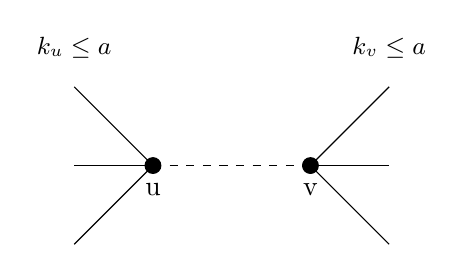
\begin{tikzpicture}
\draw [fill=black] (2,2) circle [radius=0.1];
\draw [fill=black] (4,2) circle [radius=0.1];
\node [below] at (2,1.9) {u};
\node [below] at (4,1.9) {v};
\draw [dashed] (2,2) -- (4,2);
\draw (1,1) -- (2,2);
\draw (1,2) -- (2,2);
\draw (1,3) -- (2,2);
\draw (4,2) -- (5,1);
\draw (4,2) -- (5,2);
\draw (4,2) -- (5,3);
\node at (1,3.5) {\small{$k_u\le a$}};
\node at (5,3.5) {\small{$k_v\le a$}};
\end{tikzpicture}

\begin{eqnarray*}
P(X_u=1\ \mbox{and}\ X_v=1) &=& \left[\sum_{k=0}^{a}\binom{n-2}{k}\right]^2
    \frac{1}{2}
    \left(\frac{1}{2}\right)^{k_u}\left(\frac{1}{2}\right)^{n-2-k_u}
    \left(\frac{1}{2}\right)^{k_v}\left(\frac{1}{2}\right)^{n-2-k_v} \\
    &=& \left[\sum_{k=0}^{a}\binom{n-2}{k}\right]^2
    \left(\frac{1}{2}\right)^{2n-3} \\
\end{eqnarray*}

\item{case 2: $uv\in E(G)$}

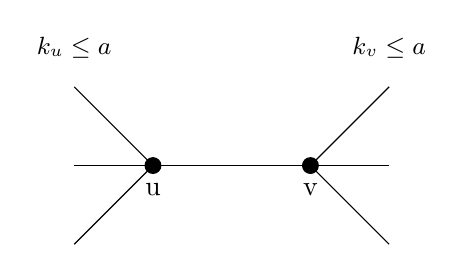
\begin{tikzpicture}
\draw [fill=black] (2,2) circle [radius=0.1];
\draw [fill=black] (4,2) circle [radius=0.1];
\node [below] at (2,1.9) {u};
\node [below] at (4,1.9) {v};
\draw (2,2) -- (4,2);
\draw (1,1) -- (2,2);
\draw (1,2) -- (2,2);
\draw (1,3) -- (2,2);
\draw (4,2) -- (5,1);
\draw (4,2) -- (5,2);
\draw (4,2) -- (5,3);
\node at (1,3.5) {\small{$k_u\le a$}};
\node at (5,3.5) {\small{$k_v\le a$}};
\end{tikzpicture}

\begin{eqnarray*}
P(X_u=1\ \mbox{and}\ X_v=1) &=& \left[\sum_{k=1}^{a}\binom{n-2}{k-1}\right]^2
    \frac{1}{2}
    \left(\frac{1}{2}\right)^{k_u}\left(\frac{1}{2}\right)^{n-2-k_u}
    \left(\frac{1}{2}\right)^{k_v}\left(\frac{1}{2}\right)^{n-2-k_v} \\
    &=& \left[\sum_{k=1}^{a}\binom{n-2}{k-1}\right]^2
    \left(\frac{1}{2}\right)^{2n-3} \\
    &=& \left[\sum_{k=0}^{a-1}\binom{n-2}{k}\right]^2
    \left(\frac{1}{2}\right)^{2n-3} \\
\end{eqnarray*}

\end{description}

\[E(X^2)=n\left(\frac{1}{2}\right)^{n-1}\sum_{k=0}^{a}\binom{n-1}{k}+
    n(n-1)\left(\frac{1}{2}\right)^{2n-3}\left\{
    \left[\sum_{k=0}^{a}\binom{n-2}{k}\right]^2+
    \left[\sum_{k=0}^{a-1}\binom{n-2}{k}\right]^2
\right\}\]

\bigskip

\item Prove $\frac{1}{2^{2m}}\binom{2m}{m}\to0$ as $m\to\infty$

\bigskip

\begin{lemma}
\[\frac{1}{2^{2m}}\binom{2m}{m}=\prod_{k=1}^{m}\left(1-\frac{1}{2k}\right)\]
\end{lemma}

\begin{theproof}[by induction on $m$]
\listbreak
\begin{description}
\item{Base:} $m=1$
\[\frac{1}{2^{2\cdot1}}\binom{2\cdot1}{1}=\frac{1}{4}\cdot2=\frac{1}{2}\]
\[\prod_{k=1}^{1}\left(1-\frac{1}{2k}\right)=1-\frac{1}{2}=\frac{1}{2}\]

\item{Assume $\frac{1}{2^{2m}}\binom{2m}{m}=
    \prod_{k=1}^{m}\left(1-\frac{1}{2k}\right)$}

\item{Consider $m+1$:}
\begin{eqnarray*}
\frac{1}{2^{2(m+1)}}\binom{2(m+1)}{m+1} &=&
    \frac{1}{2^{2m+2}}\binom{2m+2}{m+1} \\
    &=& \left(\frac{1}{2^2}\right)\left(\frac{1}{2^{2m}}\right)
    \left[\frac{(2m+2)!}{(m+1)!(m+1)!}\right] \\
    &=& \frac{1}{2^2}\left[\frac{(2m+2)(2m+1)}{(m+1)(m+1)}\right]
    \left(\frac{1}{2^{2m}}\right)\left[\frac{(2m)!}{m!m!}\right] \\
    &=& \left(\frac{2m+1}{2m+2}\right)
    \left(\frac{1}{2^{2m}}\right)\binom{2m}{m} \\
    &=& \left(\frac{2m+2-1}{2m+2}\right)
    \left(\frac{1}{2^{2m}}\right)\binom{2m}{m} \\
    &=& \left[1-\frac{1}{2(m+1)}\right]
    \prod_{k=1}^{m}\left(1-\frac{1}{2k}\right) \\
    &=& \prod_{k=1}^{m+1}\left(1-\frac{1}{2k}\right) \\
\end{eqnarray*}

\end{description}
\end{theproof}

We will also need the following anti-derivative:

\[\int\log\left(1-\frac{a}{x}\right)dx\hspace{0.25in}\mbox{(by parts)}\]

\begin{eqnarray*}
u &=& \log\left(1-\frac{a}{x}\right) \\
du &=& \frac{1}{1-\frac{a}{x}}\left(\frac{a}{x^2}\right)dx=
    \frac{a}{x^2-ax}dx \\
\\
dv &=& dx \\
v &=& x \\
\end{eqnarray*}

\begin{eqnarray*}
\int\log\left(1-\frac{a}{x}\right)dx &=&
    x\log\left(1-\frac{a}{x}\right)-a\int\frac{dx}{x-a} \\
    &=& x\log\left(1-\frac{a}{x}\right)-a\log(x-a) \\
\end{eqnarray*}

Now, let $y=\frac{1}{2^{2m}}\binom{2m}{m}$:

\begin{eqnarray*}
y &=& \prod_{k=1}^{m}\left(1-\frac{1}{2k}\right) \\
\log y &=& \sum_{k=1}^{m}\log\left(1-\frac{1}{2k}\right) \\
\end{eqnarray*}

Consider the function $f(x)=\log\left(1-\frac{1}{2x}\right)$ on $[1,m]$ in
relation to the sum:

\begin{tikzpicture}
\draw[help lines, <->] (-1,0) -- (5,0);
\draw[help lines, <->] (0,1) -- (0,-2);
\draw [fill=black] (1,{-ln(2)}) circle [radius=0.05];
\draw [domain=1:5] plot (\x, {ln(1-1/(2*\x)});
\node [below] at (1,{-ln(2)}) {\scriptsize{$(1,-log(2))$}};
\draw (1,0) rectangle (2,{-ln(2)});
\draw (2,0) rectangle (3,{-ln(4/3)});
\draw (3,0) rectangle (4,{-ln(6/5)});
\draw (4,0) rectangle (5,{-ln(8/7)});
\end{tikzpicture}

Since the function is monotonically increasing, the terms of the series
represent a lower sum for the integral:

\begin{eqnarray*}
\log y &\le& \int_{1}^{m}\log\left(1-\frac{1}{2x}\right)dx \\
    &=& \left[\log\left(1-\frac{1}{2x}\right)-
    \frac{1}{2}\log\left(x-\frac{1}{2}\right)\right]_{1}^{m} \\
    &=& \left[m\log\left(1-\frac{1}{2m}\right)-
    \frac{1}{2}\log\left(m-\frac{1}{2}\right)\right]-
    \left[\log\frac{1}{2}-\frac{1}{2}\log\frac{1}{2}\right] \\
    &=& \log\left(1-\frac{1}{2m}\right)^{m}-
    \log\sqrt{m-\frac{1}{2}}-\log\sqrt{2} \\
\end{eqnarray*}

Applying limit laws to the last line:

\[\left(1-\frac{1}{2m}\right)^{m}=
    \left\{\left[1+\left(-\frac{1}{2m}\right)
    \right]^{(-2m)}\right\}^{-\frac{1}{2}}\to e^{-\frac{1}{2}}\]
\[\log\left(1-\frac{1}{2m}\right)^{m}\to\log e^{-\frac{1}{2}}=-\frac{1}{2}\]
\[\log\sqrt{m-\frac{1}{2}}\to\infty\]
\[\log\sqrt{2}\to\log\sqrt{2}\]
\[\therefore \log y\to -\infty\ \mbox{and}\ y\to0\]

\bigskip

\item Prove that $\frac{E(X^2)}{E(X)^2}\to1$ as $n\to\infty$

\bigskip

Recall the binomial identity: $\sum_{k=0}^{m}\binom{m}{k}=2^m$, and the fact
that the binomial coefficients are symmetric:

\begin{description}
\item{m odd:}
\begin{eqnarray*}
\sum_{k=0}^{m}\binom{m}{k} &=& \binom{m}{0}+\ldots+\binom{m}{\frac{m-1}{2}}
    +\binom{m}{\frac{m+1}{2}}+\ldots+\binom{m}{m} \\
2^m &=& 2\sum_{k=0}^{\frac{m-1}{2}}\binom{m}{k} \\
\sum_{k=0}^{\frac{m-1}{2}}\binom{m}{k} &=& 2^{m-1} \\
\end{eqnarray*}

\item{m even:}
\begin{eqnarray*}
\sum_{k=0}^{m}\binom{m}{k} &=& \binom{m}{0}+\ldots+\binom{m}{\frac{m-2}{2}}
    +\binom{m}{\frac{m}{2}}
    +\binom{m}{\frac{m+2}{2}}+\ldots+\binom{m}{m} \\
2^m &=& 2\sum_{k=0}^{\frac{m}{2}}\binom{m}{k}-\binom{m}{\frac{m}{2}} \\
\sum_{k=0}^{\frac{m}{2}}\binom{m}{k} &=& 2^{m-1}+\frac{1}{2}\binom{m}{\frac{m}{2}} \\
\end{eqnarray*}
\end{description}

We can use this to replace the sums in the expressions for $E(X^2)$ and
$E(X)^2$, being careful to use the correct even/odd case:
\begin{description}
\newpage
\item{\textbf{case 1: $n$ even}}

\footnotesize\begin{eqnarray*}
\frac{E(X^2)}{E(X^2)}
&=& \frac{n\left(\frac{1}{2}\right)^{n-1}\sum_{k=0}^{\frac{n-2}{2}}\binom{n-1}{k}+
    n(n-1)\left(\frac{1}{2}\right)^{2n-3}\left\{
    \left[\sum_{k=0}^{\frac{n-2}{2}}\binom{n-2}{k}\right]^2+
    \left[\sum_{k=0}^{\frac{n-4}{2}}\binom{n-2}{k}\right]^2\right\}}
    {\left[n\left(\frac{1}{2}\right)^{n-1}\sum_{k=0}^{\frac{n-2}{2}}\binom{n-1}{k}
    \right]^2} \\
&=& \frac{n\left(\frac{1}{2}\right)^{n-1}\sum_{k=0}^{\frac{n-2}{2}}\binom{n-1}{k}+
    n(n-1)\left(\frac{1}{2}\right)^{2n-3}\left\{
    \left[\sum_{k=0}^{\frac{n-2}{2}}\binom{n-2}{k}\right]^2+
    \left[\sum_{k=0}^{\frac{n-2}{2}}\binom{n-2}{k}-
    \binom{n-2}{\frac{n-2}{2}}\right]^2\right\}}
    {\left[
    n\left(\frac{1}{2}\right)^{n-1}\sum_{k=0}^{\frac{n-2}{2}}\binom{n-1}{k}
    \right]^2} \\
&=& \frac{n\left(\frac{1}{2}\right)^{n-1}\left(2^{n-2}\right)+
    n(n-1)\left(\frac{1}{2}\right)^{2n-3}\left\{
    \left[2^{n-3}+\frac{1}{2}\binom{n-2}{\frac{n-2}{2}}\right]^2+
    \left[2^{n-3}+\frac{1}{2}\binom{n-2}{\frac{n-2}{2}}-
    \binom{n-2}{\frac{n-2}{2}}\right]^2\right\}}
    {\left[n\left(\frac{1}{2}\right)^{n-1}\left(2^{n-2}\right)\right]^2} \\
&=& \frac{\frac{n}{2}+n(n-1)\left(\frac{1}{2}\right)^{2n-3}\left\{
    \left[2^{n-3}+\frac{1}{2}\binom{n-2}{\frac{n-2}{2}}\right]^2+
    \left[2^{n-3}-\frac{1}{2}\binom{n-2}{\frac{n-2}{2}}\right]^2\right\}}
    {\left(\frac{n}{2}\right)^2} \\
&=& \frac{2}{n}+\frac{4n(n-1)}{n^2}\left(\frac{1}{2}\right)^{2n-3}\left\{
    \left[2^{n-3}+\frac{1}{2}\binom{n-2}{\frac{n-2}{2}}\right]^2+
    \left[2^{n-3}-\frac{1}{2}\binom{n-2}{\frac{n-2}{2}}\right]^2\right\} \\
&=& \frac{2}{n}+\left(\frac{n-1}{n}\right)\left(\frac{1}{2}\right)^{2n-5}\left[
    2\cdot2^{2n-6}+2\cdot\frac{1}{4}\binom{n-2}{\frac{n-2}{2}}^2\right] \\
&=& \frac{2}{n}+\left(\frac{n-1}{n}\right)\left[1+
    \left(\frac{1}{2}\right)^{2n-4}\binom{n-2}{\frac{n-2}{2}}^2\right] \\
&=& \frac{2}{n}+\left(\frac{n-1}{n}\right)\left\{1+
    \left[\left(\frac{1}{2}\right)^{n-2}\binom{n-2}{\frac{n-2}{2}}\right]^2
    \right\} \\
&\to& 0+1(1+0^2) \\
&=& 1 \\
\end{eqnarray*}
\normalsize

\newpage
\item{\textbf{case 2: $n$ odd}}

\footnotesize\begin{eqnarray*}
\frac{E(X^2)}{E(X^2)}
&=& \frac{n\left(\frac{1}{2}\right)^{n-1}\sum_{k=0}^{\frac{n-1}{2}}\binom{n-1}{k}+
    n(n-1)\left(\frac{1}{2}\right)^{2n-3}\left\{
    \left[\sum_{k=0}^{\frac{n-1}{2}}\binom{n-2}{k}\right]^2+
    \left[\sum_{k=0}^{\frac{n-3}{2}}\binom{n-2}{k}\right]^2\right\}}
    {\left[n\left(\frac{1}{2}\right)^{n-1}\sum_{k=0}^{\frac{n-1}{2}}\binom{n-1}{k}
    \right]^2} \\
&=& \frac{n\left(\frac{1}{2}\right)^{n-1}\sum_{k=0}^{\frac{n-1}{2}}\binom{n-1}{k}+
    n(n-1)\left(\frac{1}{2}\right)^{2n-3}\left\{
    \left[\sum_{k=0}^{\frac{n-3}{2}}\binom{n-2}{k}+\binom{n-2}{\frac{n-1}{2}}
    \right]^2+\left[\sum_{k=0}^{\frac{n-3}{2}}\binom{n-2}{k}\right]^2\right\}}
    {\left[n\left(\frac{1}{2}\right)^{n-1}\sum_{k=0}^{\frac{n-1}{2}}\binom{n-1}{k}
    \right]^2} \\
&=& \frac{n\left(\frac{1}{2}\right)^{n-1}\left[2^{n-2}+
    \frac{1}{2}\binom{n-1}{\frac{n-1}{2}}\right]+
    n(n-1)\left(\frac{1}{2}\right)^{2n-3}\left\{
    \left[2^{n-3}+\binom{n-2}{\frac{n-1}{2}}
    \right]^2+\left[2^{n-3}\right]^2\right\}}
    {\left\{n\left(\frac{1}{2}\right)^{n-1}\left[2^{n-2}+
    \frac{1}{2}\binom{n-1}{\frac{n-1}{2}}\right]\right\}^2} \\
&=& \frac{\frac{n}{2}\left[1+
    \left(\frac{1}{2}\right)^{n-1}\binom{n-1}{\frac{n-1}{2}}\right]+
    n(n-1)\left(\frac{1}{2}\right)^{2n-3}\left\{
    \left[2^{n-3}+\binom{n-2}{\frac{n-1}{2}}
    \right]^2+\left[2^{n-3}\right]^2\right\}}
    {\left\{\frac{n}{2}\left[1+
    \left(\frac{1}{2}\right)^{n-1}\binom{n-1}{\frac{n-1}{2}}\right]\right\}^2} \\
&=& \frac{\frac{n}{2}\left[1+
    \left(\frac{1}{2}\right)^{n-1}\binom{n-1}{\frac{n-1}{2}}\right]+
    \frac{n(n-1)}{8}\left(\frac{1}{2}\right)^{2n-6}\left\{
    \left[2^{n-3}+\binom{n-2}{\frac{n-1}{2}}
    \right]^2+\left[2^{n-3}\right]^2\right\}}
    {\left\{\frac{n}{2}\left[1+
    \left(\frac{1}{2}\right)^{n-1}\binom{n-1}{\frac{n-1}{2}}\right]\right\}^2} \\
&=& \frac{\frac{n}{2}\left[1+
    \left(\frac{1}{2}\right)^{n-1}\binom{n-1}{\frac{n-1}{2}}\right]+
    \frac{n(n-1)}{8}\left\{
    \left[1+\left(\frac{1}{2}\right)^{n-3}\binom{n-2}{\frac{n-1}{2}}
    \right]^2+1^2\right\}}
    {\left\{\frac{n}{2}\left[1+
    \left(\frac{1}{2}\right)^{n-1}\binom{n-1}{\frac{n-1}{2}}\right]\right\}^2} \\
&=& \frac{\frac{2}{n}\left[1+
    \left(\frac{1}{2}\right)^{n-1}\binom{n-1}{\frac{n-1}{2}}\right]+
    \left(\frac{n-1}{2n}\right)\left\{
    \left[1+\left(\frac{1}{2}\right)^{n-3}\binom{n-2}{\frac{n-1}{2}}
    \right]^2+1\right\}}
    {\left[1+
    \left(\frac{1}{2}\right)^{n-1}\binom{n-1}{\frac{n-1}{2}}\right]^2} \\
\end{eqnarray*}
\normalsize

Note that the $\binom{n-2}{\frac{n-1}{2}}$ term is not quite in the right form,
but we can adjust it:

\begin{eqnarray*}
\binom{n-2}{\frac{n-1}{2}} &=&
    \frac{(n-2)!}
    {\left(\frac{n-1}{2}\right)!\left(n-2-\frac{n-1}{2}\right)!} \\
&=& \left[\frac{n-1-\frac{n-1}{2}}{n-1}\right]\left[\frac{(n-1)!}
    {\left(\frac{n-1}{2}\right)!\left(n-1-\frac{n-1}{2}\right)!}\right] \\
&=& \frac{1}{2}\binom{n-1}{\frac{n-1}{2}} \\
\end{eqnarray*}

Plugging in this result and continuing, we get:

\footnotesize\begin{eqnarray*}
\frac{E(X^2)}{E(X^2)}
&=& \frac{\frac{2}{n}\left[1+
    \left(\frac{1}{2}\right)^{n-1}\binom{n-1}{\frac{n-1}{2}}\right]+
    \left(\frac{n-1}{2n}\right)\left\{
    \left[1+\left(\frac{1}{2}\right)^{n-2}\binom{n-1}{\frac{n-1}{2}}
    \right]^2+1\right\}}
    {\left[1+
    \left(\frac{1}{2}\right)^{n-1}\binom{n-1}{\frac{n-1}{2}}\right]^2} \\
&=& \frac{\frac{2}{n}\left[1+
    \left(\frac{1}{2}\right)^{n-1}\binom{n-1}{\frac{n-1}{2}}\right]+
    \left(\frac{n-1}{2n}\right)\left\{
    \left[1+2\left(\frac{1}{2}\right)^{n-1}\binom{n-1}{\frac{n-1}{2}}
    \right]^2+1\right\}}
    {\left[1+
    \left(\frac{1}{2}\right)^{n-1}\binom{n-1}{\frac{n-1}{2}}\right]^2} \\
&\to& \frac{0(1+0)+\frac{1}{2}\left[(1+2\cdot0)^2+1\right]}{(1+0)^2} \\
&=& 1 \\
\end{eqnarray*}
\normalsize
\end{description}

\bigskip

\item Prove that almost every graph has $\delta<\frac{n}{2}$

\bigskip

By Chebychev:
\[P(X=0)\le1-\frac{E(X^2)}{E(X)^2}=1-1=0\]

Therefore, there is zero probability that $X=0$, meaning that at least one
vertex must have degree $<\frac{n}{2}$.

\end{enumerate}
\end{document}
